\documentclass[12pt,a4paper]{article}
\usepackage[utf8]{inputenc}
\usepackage[english]{babel}
\usepackage{amsmath}
\usepackage{amsfonts}
\usepackage{amssymb}

\usepackage{hyperref}

\usepackage{graphicx}
\graphicspath{ {./images/} }
\usepackage{epstopdf}

\usepackage[top=1.5in, bottom=1in, left=1in, right=1in]{geometry}


% alignment of figures (H)
\usepackage{float}

% tikz graphs
\usepackage{tikz}
\usetikzlibrary{arrows,automata, positioning,calc,shapes.geometric}
\usepackage{varwidth} % for the diagram of fpga design

\usepackage{todonotes}

% for tanles
\usepackage{multirow}

% header
\usepackage{fancyhdr}
\pagestyle{fancyplain}
\fancyhf{}
\lhead{ \fancyplain{}{Lukas Schwartz \& Aitor Blanco } }
\rhead{ \fancyplain{}{EMB1 - 1. Semester MSc Robot Systems} }
\cfoot{ \fancyplain{}{\thepage} }


\begin{document}

\begin{titlepage}
	\centering
%	\includegraphics[width=0.15\textwidth]{example-image-1x1}\par\vspace{1cm}
	\vfill
	{\scshape\LARGE University of Southern Denmark\par}
	\vspace{1cm}
	{\scshape\Large EMB1 Project \#1\par}
	{\scshape\large 1. Semester MSc Robot Systems\par}
	\vspace{1.5cm}
	{\huge\bfseries Brick Sorter\par}
	\vspace{2cm}
	{\Large\itshape Aitor Miguel Blanco and Lukas Chr. M. W. Schwartz \\ Group \#1 \par}
	\vfill
	supervised by\par
	Jorgen Christian Larsen

	\vspace{2cm}

% Bottom of the page
	{\large 2$^{nd}$ November 2015 \par}
\end{titlepage}

\pagebreak

\tableofcontents

\pagebreak


\section{Introduction}

This project describes the creation of an autonomous brick sorter to sort red, green and blue Lego bricks into separate directions.
This is to be done using a slide to which there is attached a servo motor to control whether the brick is going to the left or right.
Furthermore this project considers the design of the circuits used for power supplies and   color detecting circuit.

For the control of the brick sorter a FPGA is used to control the system.
The project also requires the use of uTosNet to communicate with a computer.

This report is structured such that it first describes the hardware and schematics used.
Thereafter the program run on the FPGA is considered and finally a test of the system is conducted and a conclusion on the whole project is drawn.



%This way, the project can be easily divided in 6 different blocks,

%\begin{itemize}
%\item Power supply
%\item Light sensor.
%\item LED Control.
%\item Servo motor.
%\item PC communication.
%\item VHDL design.
%\end{itemize}
	
\pagebreak


\section{Circuit and Physical Design}
To solve the sokoban problem a robot capable of performing simple tasks concerned with moving the can and itself around the game map are needed.
The behaviours the robot should be able to perform define how the robot should be formed in order to accomplish its task of solving the sokoban problem.


\subsection{Power Supply}
The power supply has been build to deliver three different voltage levels of 5V, 6V and 12V, ensuring a current of 1A, 1.5A and 1A respectively.

This circuit has been printed in a PCB that can be plugged directly into the breadboard to deliver the required voltage and current.
The schematics of such can be seen in figure \ref{fig:powersupply_schematics}.

\begin{figure}[H]
\centering 
\includegraphics[width = 0.7 \textwidth]{images/powersupply_schematics}
\caption{Schematics of the power supply.}
\label{fig:powersupply_schematics}
\end{figure}


The power supply is connected to a 15V power supply as a input voltage. 
To convert this 15V into 12V, 6V and 5V three different elements are used.
To ensure a 5V/1A supply with a $\pm 1.5\%$ voltage for the FPGA, an LM2574 regulator is used. 
For the 6V/1.5A and 12V/1A, the 7806 and 7812 regulators are used. 
As the efficiency of these regulators is not as good as the one of the LM2574 and they dissipate the excess of power by heating up, a heat-sink for these is required.

The 7806 and 7812 both have a working temperature of maximum $125^{\circ} C$.
In order to hold the temperature of the voltage regulators below this, a heat sink able to dissipate all the heat at the maximum supply rates should be used.

The total energy dissipated by the two regulators can be found by equation \ref{eq:powersupply_energy_dissipation}.

\begin{equation}
P = V_{7806} \cdot I_{7806} + V_{7812} \cdot I_{7812} = (15 - 6) \cdot 1.5 + (15 - 12) \cdot 1 = 16.5W
\label{eq:powersupply_energy_dissipation}
\end{equation}


Estimating the surrounding temperatures to be around $25^{\circ} C$, then the heat sink must keep the temperature below $100^{\circ} C$ rise when $21W$ is dissipated.
This results in a heat sink capable of rising less than $6 ^{\circ}K/W$ is needed to cool the two regulators.
The \textit{Heatsink SK68 100mm 3K/W TO220}\footnote{\href{http://dk.rs-online.com/web/p/koleplader/1898482/?searchTerm=Heatsink+SK68+100mm+3K\%2FW+TO220&relevancy-data=636F3D3226696E3D4931384E44656661756C74266C753D6461266D6D3D6D61746368616C6C7061727469616C26706D3D5E5B5C707B4C7D5C707B4E647D5C707B5A737D2D2C2F255C2E5D2B2426706F3D3926736E3D592673743D4B4559574F52445F4D554C54495F414C5048415F4E554D455249432673633D592677633D4E4F4E45267573743D4865617473696E6B20534B3638203130306D6D20334B2F5720544F32323026}{SK68 100mm 3K/W TO220 Datasheet}} was chosen to do this.
With a $3^{\circ}K/W$ heating coefficient it should be capable of keeping the two regulators at $75^{\circ}C$ during operation with the full load and at a $25^{\circ}C$ ambient temperature.



To test the three power supplies, different loads was added to the outputs of the supplies to check if they meet the specified requirements.
The voltage supplied by the regulators was measured by an oscilloscope and the average recorded for the given load.
The results are seen in figure \ref{fig:voltagesupply}.

\begin{figure}[H]
\centering
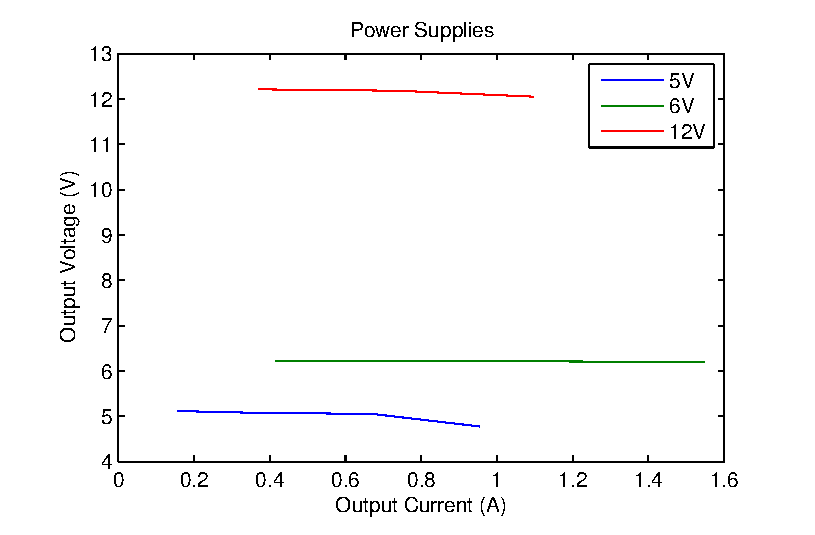
\includegraphics[width = 0.9 \textwidth]{images/powersupply_output}
\caption{Voltage output of the voltage regulators with different loads.}
\label{fig:voltagesupply}
\end{figure}

As seen in figure \ref{fig:voltagesupply} then the power supplies supply a voltage slightly less than desired when exposed to the full load, but as this decreases the voltage reaches the desired voltage.
This might not be desirable, but it is deemed good enough for the project since the power supply rarely, if at all, will be used with full load.


Furthermore the efficiency of the 5V power supply was calculated.
This was done using equation \ref{eq:powersupply_efficiency}.

\begin{equation}
Efficiency = \frac{P_{out}}{P_{in}} = \frac{V_{out}^2 / R_{out}}{V_{in} \cdot I_{in}}
\label{eq:powersupply_efficiency}
\end{equation}

Where, in equation \ref{eq:powersupply_efficiency}, V is the voltage (V), R the load ($\Omega$) and I the current (A) for the circuit where \textit{in} is what was supplied by the 15V supply and \textit{out} the output of the regulator.


\begin{table}[H]
\centering
\begin{tabular}{|c|c|c|c|c|}
\hline
Load ($\Omega$) & Min Efficiency & Avg. Efficiency & Max Efficiency \\ \hline
5 & 0.7806 & 0.7996 & 0.8367 \\ \hline
7.5 & 0.7570 & 0.8095 & 0.8096 \\ \hline
15 & 0.7556 & 0.7640 & 0.8587 \\ \hline
33 & 0.644 & 0.6607 & 0.7318 \\ \hline
\end{tabular}
\caption{Efficiency of the 5V supply.}
\label{tab:voltageefficiency}
\end{table}

The efficiency was calculated considering that the input supply is stable and using the maximum, minimum and average output voltages measured with the oscilloscope.
It can be seen from table \ref{eq:powersupply_efficiency} that the efficiency of the regulator is capable of supplying the voltages at the project requirement of 80\%, for small loads.
As the load increases above $7.5\Omega$ the efficiency decreases considerably.
This is however expectable since the regulator used specifies that the efficiency is highest when driving a load with 0.5A at 5V and then only is specified to achieve the 80\%.



\subsection{LED controller}



\begin{figure}[H]
\centering 
\includegraphics[width = 0.4 \textwidth]{images/leddriver_schematics}
\caption{...}
\label{fig:...}
\end{figure}


\subsection{Photodiode}
\label{sec:photodiode}
The photodiode is used to detect the intensity of the light shined upon it.
In operation it generates a current proportional to the intensity of the surrounding light.
This signal does, however, need to be converted into a voltage between 0 and 3.3V for the ADC to measure.

To do this, the signal is amplified using the amplifier circuit shown in figure \ref{fig:photodiodeschematics}.
The amplification was found by dimensioning the resistor such that it is close to saturation when the photodiode is exposed to the highest expected lighting level.


\begin{figure}[H]
\centering 
\includegraphics[width = 0.6 \textwidth]{images/optoamplifier_schematics}
\caption{Photodiode amplifier schematics.}
\label{fig:photodiodeschematics}
\end{figure}

As seen in figure \ref{fig:photodiodeschematics} a LM358N was chosen as the operational amplifier.
This amplifier was chosen because it is  a general purpose amplifier and no other specific requirements were needed.

The second amplifier in the package is circuited completely to ground, as seen on figure \ref{fig:photodiodeschematics}, since it is not in use.

The output of the amplifier (PHD, in figure \ref{fig:photodiodeschematics}) is then routed directly to the ADC port (OPTO, in figure \ref{fig:adc_schematics}).


\begin{figure}[H]
\centering 
\includegraphics[width = 0.4 \textwidth]{images/ADC_schematics}
\caption{Schematics of the ADC connections.}
\label{fig:adc_schematics}
\end{figure}


To test the final signal of the photodiode circuit, then the output of amplifier was compared to the output of the LEDs when these are turned on and off one after the other.
The result of such is seen in figure \ref{fig:photodiode_output}.
It can be seen on figure \ref{fig:photodiode_output} that when the LED's switch color, this results in oscillations about the resulting voltage.
When sampled at this time the data would hence be wrong.
This problem can be solved by adding a low-pass filter to the amplifier circuit to reduce/remove the oscillations or one could wait with sampling the signal until it has stabilized.
Of these two options the latter was used.
This was chosen because the number of samples gathered a second, even when not being able to sample directly after the LED has turned on, is still so high that the sample frequency is a problem.
The sample for each color is hence first taken $3.3 \cdot 10^-5 s$ after the LED is turned on.


\begin{figure}[H]
\centering 
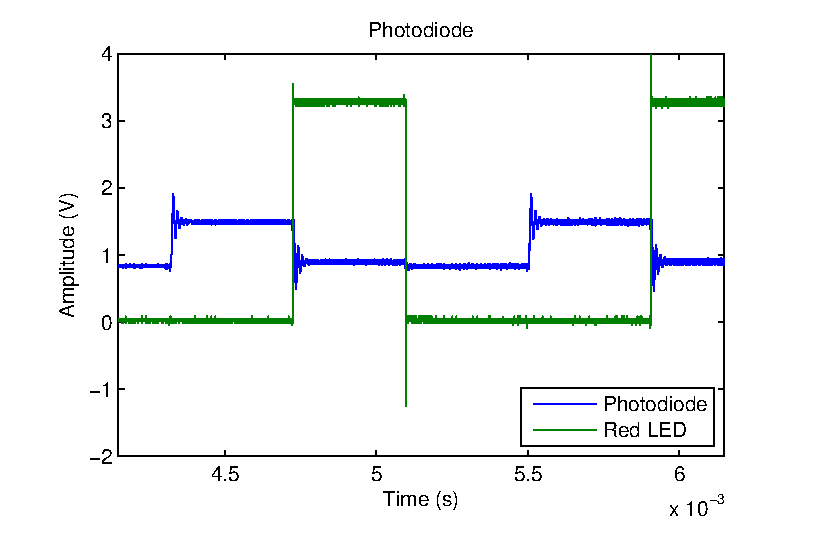
\includegraphics[width = 0.9 \textwidth]{images/photodiode}
\caption{Output of the photodiode amplification versus the signal to the red LED.}
\label{fig:photodiode_output}
\end{figure}








\pagebreak
\section{Software}
This section describes the software used to control the brick sorting system.
First the top module is described and from there the individual components are considered.

The main components and their interface is shown in figure \ref{fig:program_design}.
Apart from the shown connections in figure \ref{fig:program_design}, then a set of connections to transfer variables which can be set from the computer and the clock signal.


\begin{figure}[H]
\centering
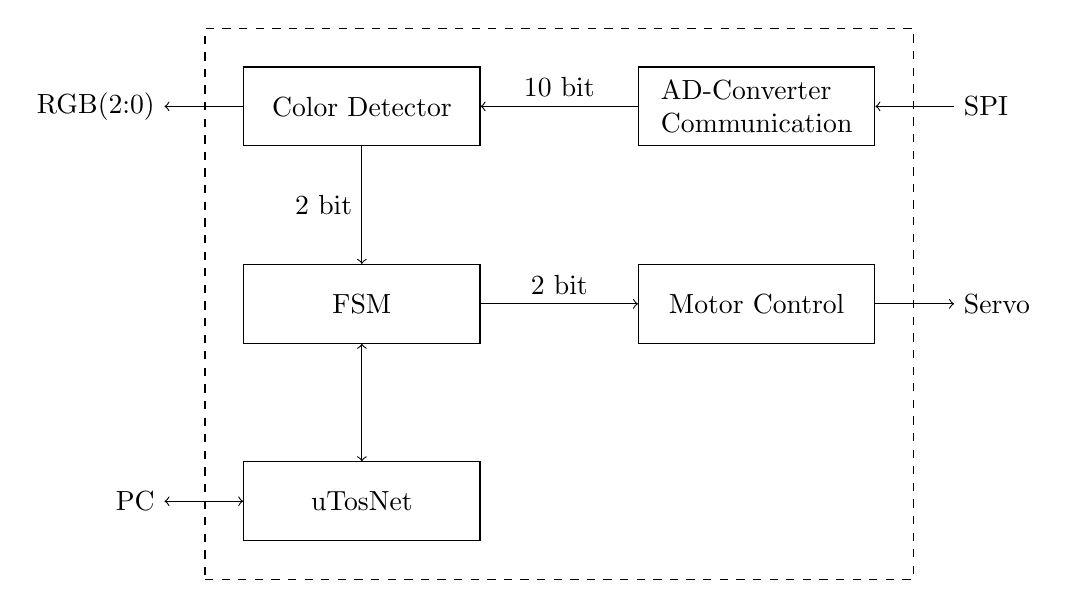
\begin{tikzpicture}[node distance=1cm]
% FPGA border
\node[rectangle,draw,minimum width=9cm, minimum height=7cm, dashed, name=FPGA]  {};

% used to align the insides of FPGA
\node[rectangle,minimum width=5cm, minimum height=5cm, name=FPGAaligne] {};

% components of FPGA
\node[rectangle,draw,minimum width=3cm, minimum height=1cm, name=utos] at (FPGAaligne.-135) {uTosNet};
\node[rectangle,draw,minimum width=3cm, minimum height=1cm, name=ad] at (FPGAaligne.45) {\begin{varwidth}{4cm}AD-Converter\\ Communication\end{varwidth}};
\node[rectangle,draw,minimum width=3cm, minimum height=1cm, name=mc] at (FPGAaligne.0) {Motor Control};
\node[rectangle,draw,minimum width=3cm, minimum height=1cm, name=fsm] at (FPGAaligne.180) {FSM};
\node[rectangle,draw,minimum width=3cm, minimum height=1cm, name=color] at (FPGAaligne.135) {Color Detector};

% nodes outside FPGA
\node [left=of utos,name=pc] {PC};
\node [right=of ad,name=adc] {SPI};
\node [left=of color,name=rgb] {RGB(2:0)};
\node [right=of mc,name=servo] {Servo};

% arrows inside FPGA
\draw[<->] (utos) -- node[] {} (fsm) ;
\draw[<-] (color) -- node[above] {10 bit} (ad) ;
\draw[->] (fsm) --  node[above] {2 bit} (mc) ;
\draw[->] (color) -- node[left] {2 bit} (fsm) ;
 
% arrows connected to the outside of FPGA
\draw[<->] (utos) to[out=180, in=0] node[] {} (pc) ;
\draw[->] (adc) to[out=180, in=0] node[] {} (ad) ;
\draw[->] (color) to[out=180, in=0] node[] {} (rgb) ;
\draw[->] (mc) to[out=0, in=180] node[] {} (servo) ;
\end{tikzpicture}

\caption{FPGA Program Design.}
\label{fig:program_design}
\end{figure}



The components of figure \ref{fig:program_design} are responsible for the following tasks.

\paragraph*{FSM}
The \textit{FSM} component is the top module of the system.
It connects the remaining components functionality in order to sort the bricks depending on their color and communicate with the computer.

\paragraph*{Color Detector}
The \textit{Color Detector} is responsible for controlling the LEDs and use the data from the ADC to decide the color of the bricks passing through the system.
This way it is able to connect the light intensity values from the photo-diode and relate them to a specific color.
From there the data is used to decide which brick, if any, is passing the sensor.

\paragraph*{AD-converter Communication}
This component implements the SPI communication to the ADC and feeds this onwards to the \textit{Color Detector}.


\paragraph*{Motor Control}
The \textit{Motor Control} component is controlling the servo motor using an input signal, deciding which of three positions it should be in.
Either the left- or right-tray or the idle position.

\paragraph*{uTosNet}
UTosNet is the component supplied by SDU which implements the communication with the computer.
This component is hence created such that it is capable of transferring data of importance to the FPGA and change specific settings or gather data from such.





\subsection{Top Module}
The top module is the part of the system which combines all the functionality the FPGA should have.
Its core functionality is implemented as the state machine in figure \ref{fig:topmodule_fsm}.
This state machine is sorting the bricks using the signals generated from the sub components.


\begin{figure}[H]
\centering
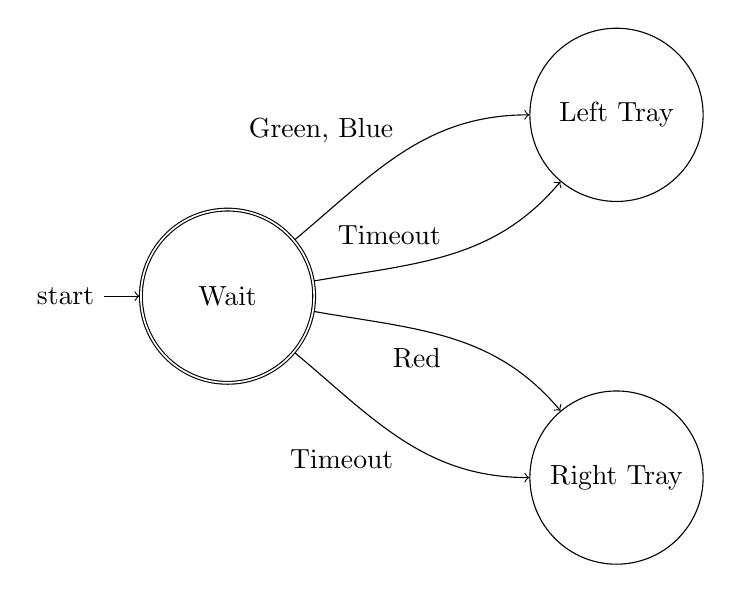
\begin{tikzpicture}[node distance=3cm]
\node[circle, minimum width=6cm, name=c] {};

\node[initial,accepting,state,name=start,minimum width=2.2cm] at (c.180)   {Wait}; 

\node[state,name=left,minimum width=2.2cm] at (c.50)   {Left Tray}; 
\node[state,name=right,minimum width=2.2cm] at (c.-50)   {Right Tray}; 


%\node[name=rst] at (-2.5,3) {rst};

\draw[->] (start) to[out=40, in=180] node[midway,above left] {Green, Blue} (left) ;
\draw[->] (start) to[out=10, in=230] node[midway,above left] {Timeout} (left) ;

\draw[->] (start) to[out=-10, in=-230] node[midway,below left] {Red} (right) ;
\draw[->] (start) to[out=-40, in=180] node[midway,below left] {Timeout} (right) ;  
\end{tikzpicture}

\caption{Top module Finite State Machine.}
\label{fig:topmodule_fsm}
\end{figure}


The state machine in figure \ref{fig:topmodule_fsm} waits in the idle mode whenever no brick is or has passed.
When a brick is detected, and the state machine is in the \textit{Wait} state, then it moves to the \textit{Right-} or \textit{Left Tray} state depending on the color of the brick.
When the state is changed, a timer is started and this generated a timeout signal once the time has elapsed.
This timeout results in the state machine returning to its initial \textit{Wait} state when the brick has passed the sorter.
While the state machine is in \textit{Left-} or \textit{Right Tray}, it sends a signal to the \textit{Motor Control} component to move to the left or right side in order to sort the bricks.
Otherwise, the motors are told to return to its initial position, which is when the motor is pointing the sorter towards the falling bricks.
The timeout period before switching back to the \textit{Wait} state was set such that the bricks would have enough time to pass through the sorting mechanism on the slide before the sorter would return to its initial state.




\subsection{AD-Converter Communication}
The ADC communicates using SPI.
This is hence implemented in the module.
Since the ADC only allows up to 3.6MHz communication frequency, then the clock is scaled down to 3.57MHz.
The FPGA is then requesting the data from the ADC continuously and whenever a whole message is received, it is send out into the FPGA and a signal is pulsed to notify the color detector of the new message.

\subsection{Color Detector}
The color detector is responsible for figuring out which, if any, brick color passes by the sensor.
It does this by using both input from the ADC Communication and by controlling the three different colors of LEDs.

The color detector component is designed as the state machine in figure \ref{fig:colordetector_fsm}.


\todo[inline]{make this state diagram, this is the wrong one!}

\begin{figure}[H]
\centering
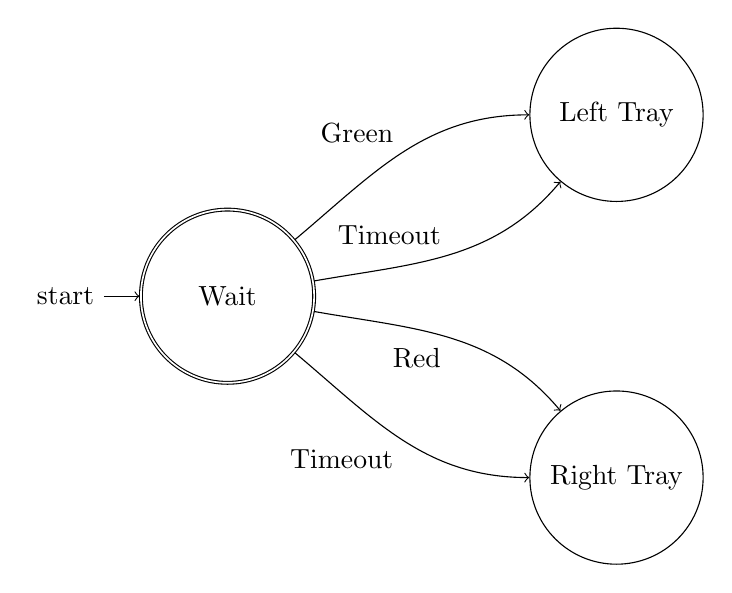
\begin{tikzpicture}[node distance=3cm]
\node[circle, minimum width=6cm, name=c] {};

\node[initial,accepting,state,name=start,minimum width=2.2cm] at (c.180)   {Wait}; 

\node[state,name=left,minimum width=2.2cm] at (c.50)   {Left Tray}; 
\node[state,name=right,minimum width=2.2cm] at (c.-50)   {Right Tray}; 


%\node[name=rst] at (-2.5,3) {rst};

\draw[->] (start) to[out=40, in=180] node[midway,above left] {Green} (left) ;
\draw[->] (start) to[out=10, in=230] node[midway,above left] {Timeout} (left) ;

\draw[->] (start) to[out=-10, in=-230] node[midway,below left] {Red} (right) ;
\draw[->] (start) to[out=-40, in=180] node[midway,below left] {Timeout} (right) ;  
\end{tikzpicture}

\caption{Color detectors Finite State Machine.}
\label{fig:colordetector_fsm}
\end{figure}




\subsection{Servo Motor}
The servo motor is controlled by giving it a command to which of three positions it has to go.
The three positions are left, right and center.
The specific value to which it moves is made adjustable from the computer by setting a 9 bit signal for each of the three positions.
This generates a timing between approximately 1 and 2 ms.




\subsection{PC Communication}
The communication to the PC...

\pagebreak
\section{Test of the System}
The final system was tested to see how well it performs.
The tests where performed in normal ambient light and with the thresholds set beforehand to a suitable value.

A set of bricks where let slide through the setup and the result shown in the confusion table in table \ref{tab:confusiontable_testresults}.


\begin{table}[H]
\centering
\begin{tabular}{|c|c|c|c|c|}
\hline
 & &  \multicolumn{3}{|c|}{Predicted} \\ \hline
 & & Red & Green & Blue \\ \cline{1-5} 
\multirow{3}{*}{Actual} & Red & & & \\ \cline{2-5}
 & Green & & & \\ \cline{2-5}
 & Blue & & & \\ \hline
\end{tabular}
\caption{Confusion table of the test results.}
\label{tab:confusiontable_testresults}
\end{table}

\pagebreak
\section{Conclusion}

After building the robot and testing all the implemented behaviours, it was found that the proposed solution is robust enough to execute any given path.
The robot works under different ambient light levels due to a mounted shield that shadows the sensors, making them less sensitive to external light.
The robot can run for over 30 minutes without problems from having a low battery level.

To find a solution for the Sokoban problem an A* algorithm has been devised.
Using the diamond pushes as nodes and the number of steps of the robot to achieve a certain state as the cost.
The algorithm uses, as heuristics, the cost of moving each diamond from their position to the nearest goal when having to push them around the walls in a else completely empty map.
The nodes in the graph are validated using the diamonds and robots state.
The individual states are checked for deadlock situations to reduce the graph.

The solver can work for any map satisfying a constrained map size.

To load the generated path into the robot, a path converter was implemented.
This function can convert the generated path to be executable for the robot.

By combining the two parts of this project, it is possible to load a certain sokoban map, find a solution for it and solve physically the challenge with the robot.






\end{document}